
\documentclass[border=10pt, 12pt]{standalone}
\usepackage[svgnames]{xcolor}
\usepackage{amsmath}
\usepackage{pgfplots}
\pgfplotsset{compat=newest}
\usepackage[sfdefault]{FiraSans}
\usepackage{FiraMono}
\renewcommand*\familydefault{\sfdefault}
\begin{document}
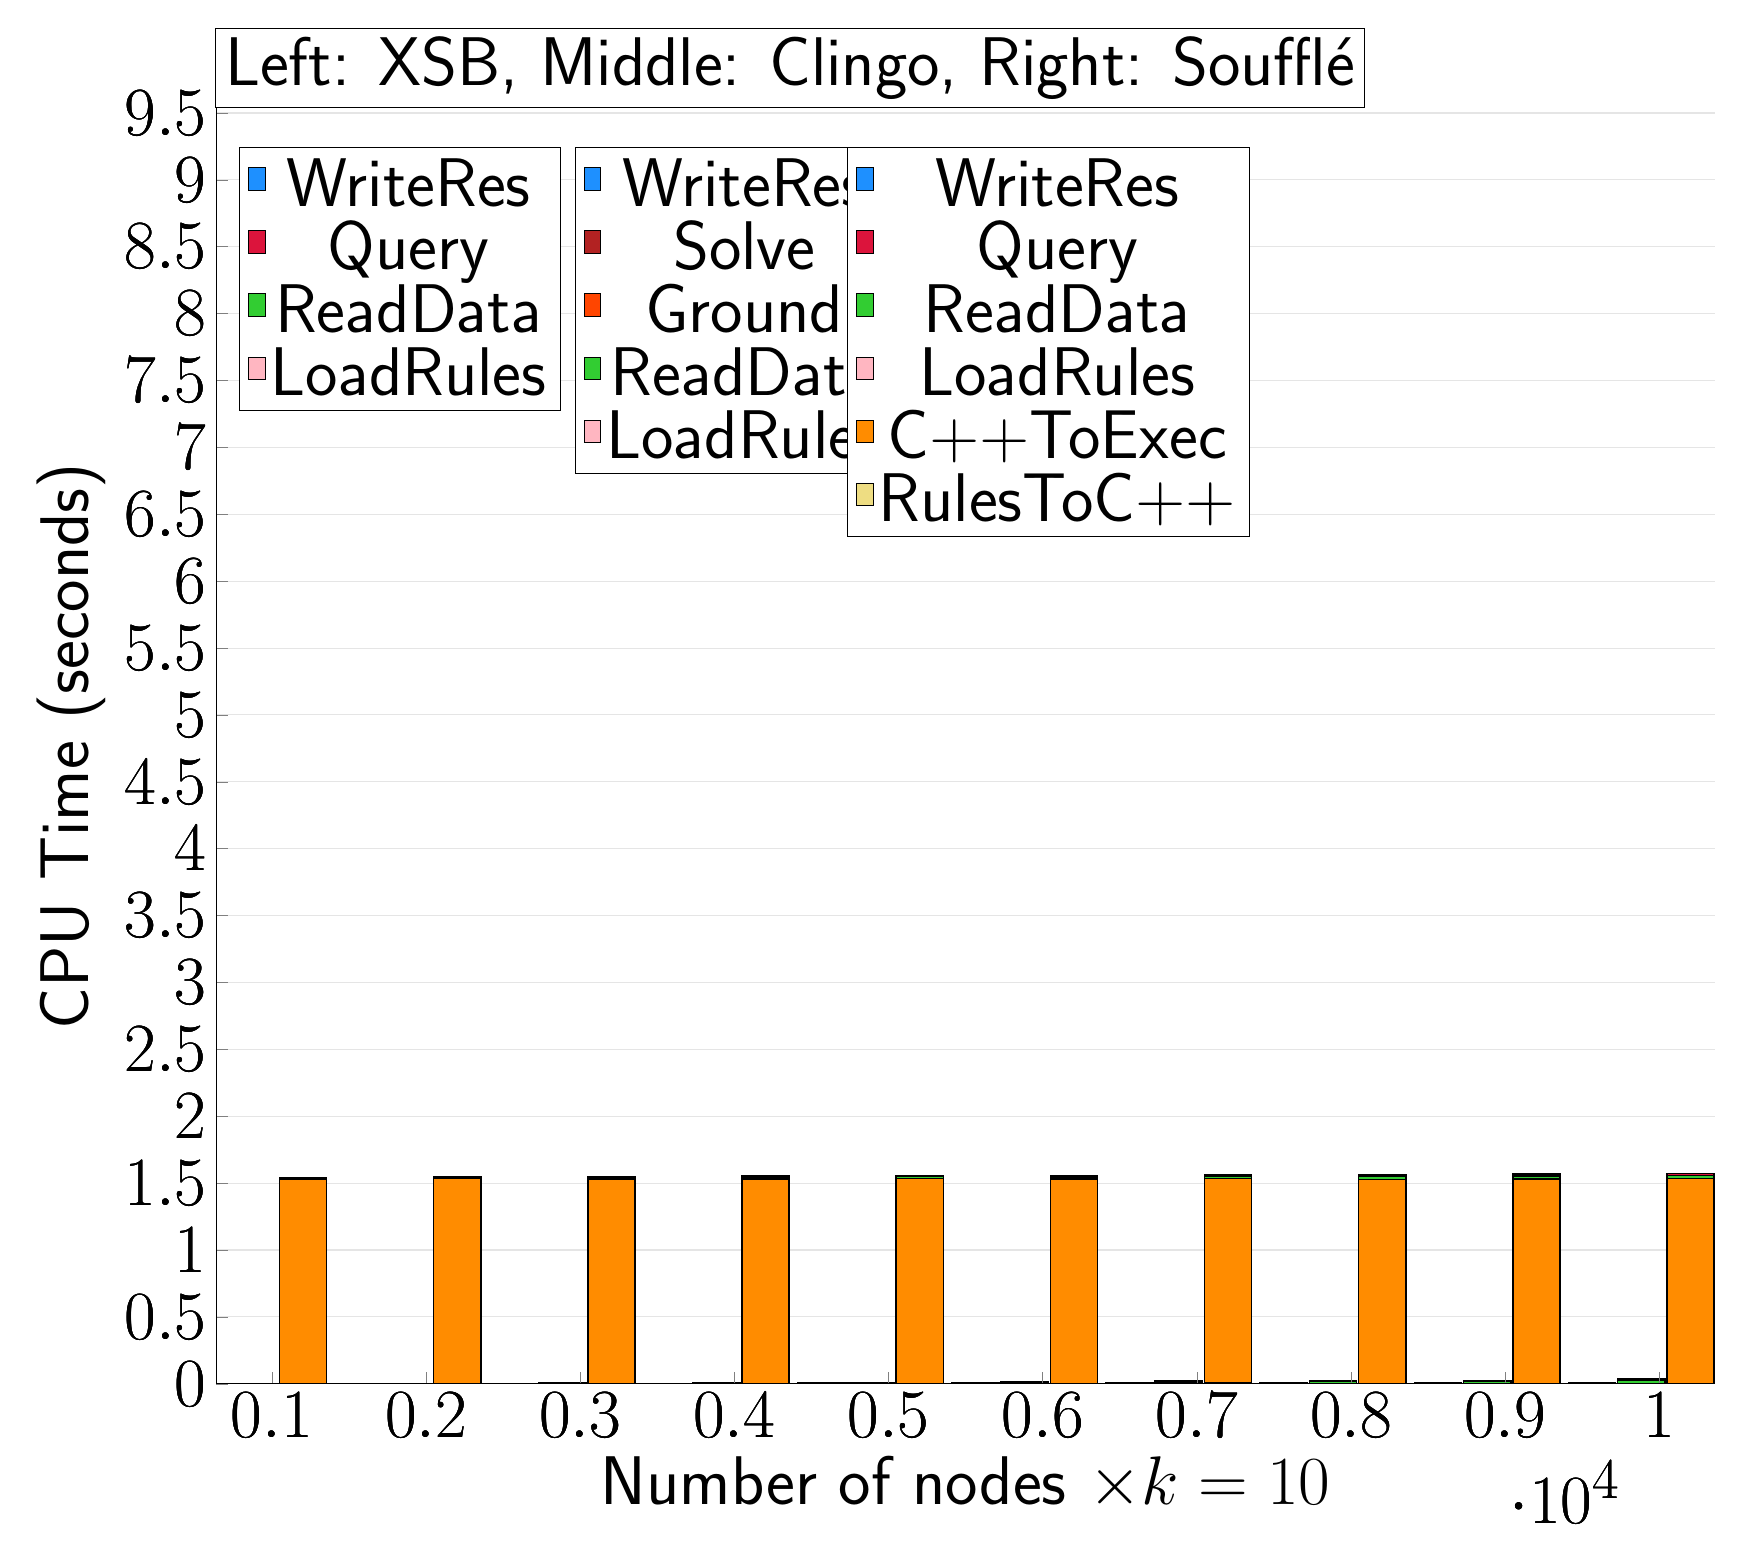
\begin{tikzpicture}
                        \begin{axis}[bar shift=-24.3pt, 
   ybar stacked,
   width=1.7\textwidth,
   bar width=0.6cm,
   ymajorgrids, tick align=inside,
   major grid style={draw=gray!20},
   xtick=data,
   ymin=0, ymax=9.534,
   axis x line*=bottom,
   axis y line*=left,
   enlarge x limits=0.04,
   legend style={
       at={(0.23, 0.97)},
       anchor=north east,
       legend columns=1,
       font=\Huge,
   },
   ylabel={CPU Time (seconds)},
   xlabel={Number of nodes $\times k=10$},
   label style={font=\Huge},
   tick label style={font=\Huge},
]
\addlegendimage{fill=DodgerBlue, draw=black, line width=0.2pt}
\addlegendentry{WriteRes}
\addlegendimage{fill=Crimson, draw=black, line width=0.2pt}
\addlegendentry{Query}
\addlegendimage{fill=LimeGreen, draw=black, line width=0.2pt}
\addlegendentry{ReadData}
\addlegendimage{fill=LightPink, draw=black, line width=0.2pt}
\addlegendentry{LoadRules}
\addplot +[fill=LightPink, draw=black, line width=0.55pt] coordinates {
(1000, 0.0005530000000000003)
(2000, 0.0005596000000000002)
(3000, 0.0005542)
(4000, 0.0005555999999999998)
(5000, 0.0005520000000000004)
(6000, 0.0005492)
(7000, 0.0005513999999999996)
(8000, 0.0005546)
(9000, 0.0005670000000000004)
(10000, 0.0005534000000000004)
};
\addplot +[fill=LimeGreen, draw=black, line width=0.55pt] coordinates {
(1000, 0.0008905999999999994)
(2000, 0.0016815999999999997)
(3000, 0.0024896000000000002)
(4000, 0.0032626)
(5000, 0.004072)
(6000, 0.0049254)
(7000, 0.0056962)
(8000, 0.006597799999999999)
(9000, 0.0074544)
(10000, 0.0082246)
};
\addplot +[fill=Crimson, draw=black, line width=0.55pt] coordinates {
(1000, 1.1000000000000598e-05)
(2000, 1.0599999999999854e-05)
(3000, 1.0199999999999792e-05)
(4000, 1.3400000000000199e-05)
(5000, 1.13999999999989e-05)
(6000, 1.2199999999999697e-05)
(7000, 1.0799999999999698e-05)
(8000, 1.1799999999999999e-05)
(9000, 1.2799999999998219e-05)
(10000, 1.21999999999983e-05)
};
\addplot +[fill=DodgerBlue, draw=black, line width=0.55pt] coordinates {
(1000, 6.399999999999913e-05)
(2000, 6.439999999999983e-05)
(3000, 6.54000000000005e-05)
(4000, 6.180000000000038e-05)
(5000, 6.32000000000011e-05)
(6000, 6.280000000000036e-05)
(7000, 6.360000000000011e-05)
(8000, 6.399999999999982e-05)
(9000, 6.480000000000133e-05)
(10000, 6.340000000000099e-05)
};
\end{axis}

\begin{axis}[bar shift=-6.5pt, 
   ybar stacked,
   width=1.7\textwidth,
   bar width=0.6cm,
   ymajorgrids, tick align=inside,
   major grid style={draw=none},
   xtick=data,
   ymin=0, ymax=9.534,
   axis x line*=none,
   axis y line*=none,
   enlarge x limits=0.04,
   legend style={
       at={(0.454, 0.97)},
       anchor=north east,
       legend columns=1,
       font=\Huge,
   },
   label style={font=\Huge},
   tick label style={font=\Huge},
]
\addlegendimage{fill=DodgerBlue, draw=black, line width=0.2pt}
\addlegendentry{WriteRes}
\addlegendimage{fill=FireBrick, draw=black, line width=0.2pt}
\addlegendentry{Solve}
\addlegendimage{fill=OrangeRed, draw=black, line width=0.2pt}
\addlegendentry{Ground}
\addlegendimage{fill=LimeGreen, draw=black, line width=0.2pt}
\addlegendentry{ReadData}
\addlegendimage{fill=LightPink, draw=black, line width=0.2pt}
\addlegendentry{LoadRules}
\addplot +[fill=LightPink, draw=black, line width=0.55pt] coordinates {
(1000, 0.0)
(2000, 0.0)
(3000, 0.0)
(4000, 0.0)
(5000, 0.0)
(6000, 0.0)
(7000, 0.0)
(8000, 0.0)
(9000, 0.0)
(10000, 0.0)
};
\addplot +[fill=LimeGreen, draw=black, line width=0.55pt] coordinates {
(1000, 0.0)
(2000, 0.0)
(3000, 0.008000000000000007)
(4000, 0.010000000000000009)
(5000, 0.010000000000000009)
(6000, 0.01200000000000001)
(7000, 0.014000000000000012)
(8000, 0.020000000000000018)
(9000, 0.020000000000000018)
(10000, 0.026000000000000023)
};
\addplot +[fill=OrangeRed, draw=black, line width=0.55pt] coordinates {
(1000, 0.0)
(2000, 0.0020000000000000018)
(3000, 0.0020000000000000018)
(4000, 0.0)
(5000, 0.0)
(6000, 0.006000000000000005)
(7000, 0.006000000000000005)
(8000, 0.0020000000000000018)
(9000, 0.0020000000000000018)
(10000, 0.009999999999999998)
};
\addplot +[fill=FireBrick, draw=black, line width=0.55pt] coordinates {
(1000, 0.0)
(2000, 0.0020000000000000018)
(3000, 0.0)
(4000, 0.0)
(5000, 0.0)
(6000, 0.0)
(7000, 0.0)
(8000, 0.0)
(9000, 0.0)
(10000, 0.0)
};
\addplot +[fill=DodgerBlue, draw=black, line width=0.55pt] coordinates {
(1000, 0.0)
(2000, -0.0020000000000000018)
(3000, 0.0)
(4000, 0.0)
(5000, 0.0)
(6000, 0.0)
(7000, 0.0)
(8000, 0.0)
(9000, 0.0)
(10000, 0.0)
};
\end{axis}

\begin{axis}[bar shift=11.3pt, 
   ybar stacked,
   width=1.7\textwidth,
   bar width=0.6cm,
   ymajorgrids, tick align=inside,
   major grid style={draw=none},
   xtick=data,
   ymin=0, ymax=9.534,
   axis x line*=none,
   axis y line*=none,
   enlarge x limits=0.04,
   legend style={
       at={(0.69, 0.97)},
       anchor=north east,
       legend columns=1,
       font=\Huge,
   },
   label style={font=\Huge},
   tick label style={font=\Huge},
]
\addlegendimage{fill=DodgerBlue, draw=black, line width=0.2pt}
\addlegendentry{WriteRes}
\addlegendimage{fill=Crimson, draw=black, line width=0.2pt}
\addlegendentry{Query}
\addlegendimage{fill=LimeGreen, draw=black, line width=0.2pt}
\addlegendentry{ReadData}
\addlegendimage{fill=LightPink, draw=black, line width=0.2pt}
\addlegendentry{LoadRules}
\addlegendimage{fill=DarkOrange, draw=black, line width=0.2pt}
\addlegendentry{C++ToExec}
\addlegendimage{fill=LightGoldenrod, draw=black, line width=0.2pt}
\addlegendentry{RulesToC++}
\addplot +[fill=LightGoldenrod, draw=black, line width=0.55pt] coordinates {
(1000, 0.0)
(2000, 0.0)
(3000, 0.0020000000000000005)
(4000, 0.0)
(5000, 0.0)
(6000, 0.0020000000000000005)
(7000, 0.006000000000000001)
(8000, 0.0)
(9000, 0.0020000000000000005)
(10000, 0.0020000000000000005)
};
\addplot +[fill=DarkOrange, draw=black, line width=0.55pt] coordinates {
(1000, 1.532)
(2000, 1.5340000000000003)
(3000, 1.528)
(4000, 1.532)
(5000, 1.534)
(6000, 1.53)
(7000, 1.53)
(8000, 1.528)
(9000, 1.53)
(10000, 1.532)
};
\addplot +[fill=LightPink, draw=black, line width=0.55pt] coordinates {
(1000, 0.0001702)
(2000, 0.0001624)
(3000, 0.0001562)
(4000, 0.00017040000000000002)
(5000, 0.00015759999999999998)
(6000, 0.00013220000000000001)
(7000, 0.00015179999999999998)
(8000, 0.0001578)
(9000, 0.0001568)
(10000, 0.0001732)
};
\addplot +[fill=LimeGreen, draw=black, line width=0.55pt] coordinates {
(1000, 0.004194)
(2000, 0.0069178)
(3000, 0.0088824)
(4000, 0.011866999999999999)
(5000, 0.0145922)
(6000, 0.014802399999999999)
(7000, 0.0174332)
(8000, 0.0203816)
(9000, 0.023132200000000002)
(10000, 0.023914200000000004)
};
\addplot +[fill=Crimson, draw=black, line width=0.55pt] coordinates {
(1000, 0.0025572)
(2000, 0.004063800000000001)
(3000, 0.0055176)
(4000, 0.0076806)
(5000, 0.00895)
(6000, 0.0093322)
(7000, 0.011400799999999999)
(8000, 0.012695999999999999)
(9000, 0.012908)
(10000, 0.014492399999999999)
};
\addplot +[fill=DodgerBlue, draw=black, line width=0.55pt] coordinates {
(1000, 0.0003981999999999999)
(2000, 0.0003012)
(3000, 0.00027400000000000005)
(4000, 0.0002478)
(5000, 0.00023880000000000003)
(6000, 0.00023859999999999997)
(7000, 0.0002326)
(8000, 0.0002448)
(9000, 0.0002376)
(10000, 0.0002222)
};
\end{axis}


\node[anchor=south, draw, fill=white] at (rel axis cs:0.42,1) {\Huge Left: XSB, Middle: Clingo, Right: Soufflé};
\end{tikzpicture}
\end{document}
                    